\newpage
\section{Durchführung}
\label{sec:Durchführung}
Während dieses Experimentes befinden sich alle Bestandteile auf einer Schiene,
damit die relativen Abstände variiert werden können. Der gesamte Aufbau ist in
Abbildung \ref{fig:Versuchsaufbau1} abgebildet. Der Aufbau besteht aus einem
Laserrohr mit aktivem Lasermedium, welcher im Laufe des Experiments zum lasen gebracht werden soll.
Zwei Resonatorspiegel sind vor und hinter dem Laserrohr angebracht, welche durch
Schrauben justiert werden können. Desweiteren befindet sich außerhalb ein
Justierlaser samt Blende. Nicht dargestellt ist eine Photodiode mit angeschlossenem
Amperemeter.
\begin{figure}[htb]
  \centering
  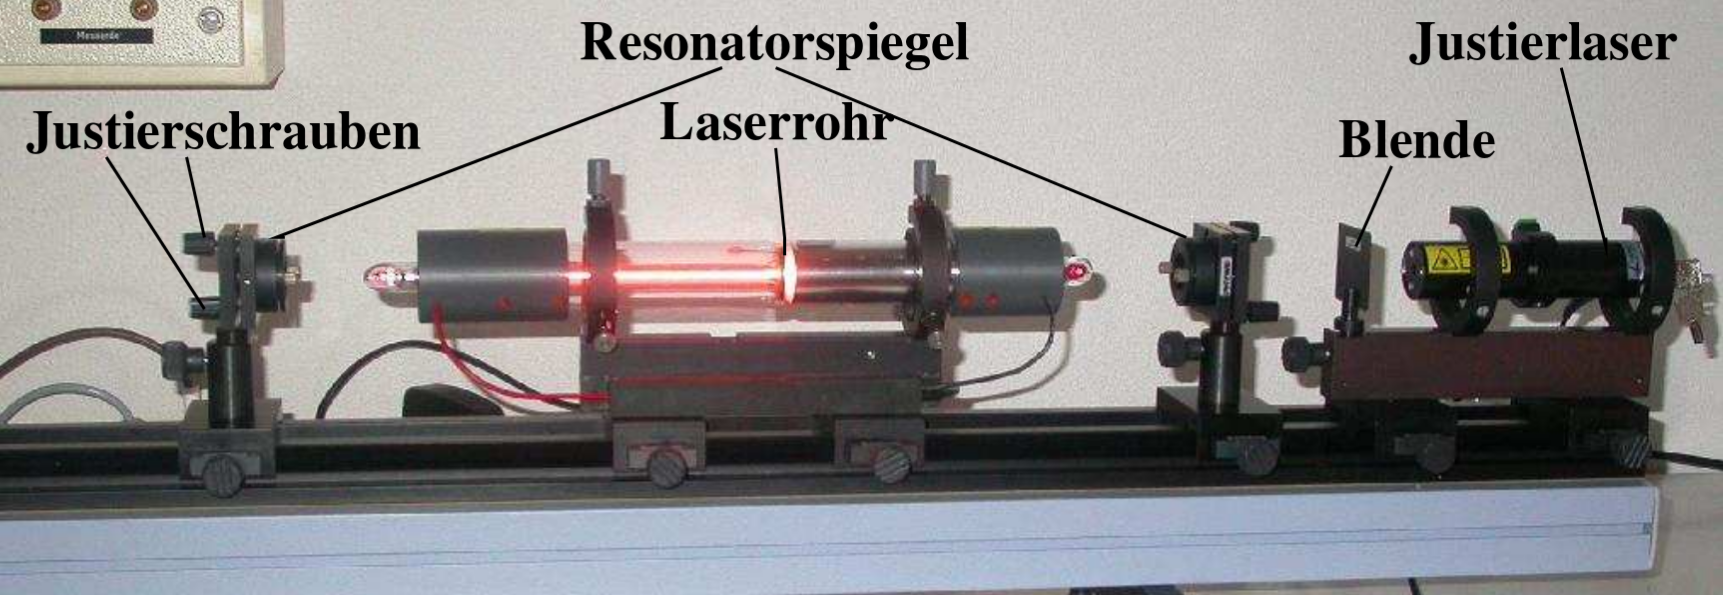
\includegraphics[width=0.8\textwidth]{content/aufbau.png}
  \caption{Aufbau eines HeNe-Lasers mit Justagelaser \cite{anleitung}.}
  \label{fig:Versuchsaufbau1}
\end{figure}
\FloatBarrier

\subsection{Justage}

Zunächst müssen die einzelnen Bestandteile justiert werden.
Zu diesem Zweck wird ein weiterer Laser und zwei Lochblenden verwendet.
Um die notwendige Gasentladung zu erhalten, wird eine Hochspannung an das Laserrohr
angelegt. Um nun den Laser zum lasen zu bringen, werden die konfokalen
Resonatorspiegel mit Justierschrauben an Spiegeln und Laserrohr so eingestellt,
dass alle optischen Achsen aufeinander liegen. Dabei ist eine Photodiode zu
Intensitätsmessung hinter dem Laser angebracht.

\subsection{Bestimmung der Wellenlänge}
Um die Wellenlänge
des erzeugten Lasers zu messen, wird ein optisches Gitter verwendet um eine
Interferenz zu erzeugen.
Zur Vermessung des entstehenden Interferenzbildes wird hinter das Gitter ein
Schirm gestellt, an dem die Abstände zwischen den auftretenden
Interferrenzmaxima vermessen werden können. Aus diesen Abständen und aus der
Messung des Abstandes zwischen Schirm und Gitter kann die Wellenlänge durch
\begin{equation}
  \lambda = \frac{g\cdot\sin(\phi)}{n},\ \ \phi = \arctan\left(\frac{d_\text{n}}{L}\right),\  n\in\mathds{N}
  \label{eqn:welle}
\end{equation}
berechnet werden. Hierbei ist $g$ die Gitterkonstante, $d_\text{n}$ der Abstand
zwischen Hauptmaxima und $n$-ten Maximum und $L$ der Abstand zwischen Gitter und
Schirm.

\subsection{Unteruchung der TEM-Moden}
Zur Untersuchung der TEM-Moden wird eine defokussierende Linse hinter dem Laser
angebracht.
Durch diese Linse wird der Strahl des Lasers verbreitert und die Untersuchung
erleichtert.
Um die Photodiode senkrecht zu der Strahlenachse verschieben zu können, wird eine
Mikrometerschraube verwendet. Durch Verschieben der Photodiode kann
die Intensität in Abhängigkeit des Achsenabstands bestimmt werden.

Die Grundmode ist ohne Einsatz von Blenden und Gittern zu untersuchen.
Die Grundmode $I_{00}$ besitzt ein Intensitätsmaximum bei $r = 0$
und wird durch Verschieben der Photodiode senkrecht zur Strahlenachse
untersucht.
Die $I_{01}$-Mode wird vermessen,
indem ein Wolframdraht zwischen den Resonatorspiegeln positioniert wird,
wodurch die Grundmode unterdrückt wird.


\subsection{Untersuchung der Polarisation}
Zur Polarisation des emittierten Laserstrahls sind an den Ausgängen des
Laserrohres Brewster-Fenster angebracht.
Diese Fenster sind gläsernde Platten, die im Brewsterwinkel bezüglich der
optischen Achse angebracht sind.
Als Brewsterwinkel wird jener Winkel bezeichnet,
bei dem (nach den Fresnelschen Formel) zur
Einfallsebene kein parallel polarisertes Licht reflektiert wird.
Zudem wird das senkrecht zur Einfallsebene polarisierte Licht
durch Reflexion stark unterdrückt.
Somit ist der verbleibende Lichtstrahl linear polarisiert.
Um diese lineare Polarisation zu überprüfen, wird zwischen die Photodiode
und den Laser ein Polarisationsfilter eingefügt.
Dieser ist drehbar gelagert, sodass die Intensität des Laserlichtes in
Abhängigkeit des Drehwinkels des Filter aufgenommen werden kann.

Das Gesetz von Malus beschreibt die Intensität des Strahls für verschiedene
Drehwinkel des Polarisationsfilters $\phi$ bezüglich der Polarisationsrichtung
des Lasers.
Es gilt der Zusammenhang
\begin{equation}
  I\left(\phi\right) = I_0 \sin^2 \left(\phi + \phi_0\right)
  \label{eqn:pol}
\end{equation}
mit der Amplitude $I_0$ und einer Phasenverschiebung $\phi_0$.

\subsection{Überprüfung der Stabilitätsbedingung}
Damit die Richtigkeit der Stabilitätsbedingung überprüft werden kann, wird die
Resonatorlänge $L$ gegen den Photostrom aufgezeichnet. Die Resonatorlänge wird
dabei auf unterschiedliche Länge eingestellt um Aussagen über die Stabilität
liefern zu können. Um Unterschiede zwischen verschiedenen Krümmungen der
Resonatorspiegel zu betrachten,
werden ein gekrümmter Spiegel $r=\SI{1.4}{\metre}$ und ein ebener Spiegel, sowie
zwei konkave Spiegel verwendet.
Bei jeder Variation der Resonatorlänge ist dabei die Justage neu durchzuführen,
um den Photostrom zu maximieren.
